\documentclass{sidenotes-simplex}
\usepackage{graphicx,longtable,calc,etoolbox,caption}
\RenewDocumentEnvironment{wideblock}{}{\begin{adjustwidth}{0mm}{-54mm}\setlength{\hsize}{\linewidth}\setlength{\columnwidth}{\linewidth}}{\end{adjustwidth}}
\providecommand{\tightlist}{\setlength{\itemsep}{0pt}\setlength{\parskip}{0pt}}
\providecommand{\passthrough}[1]{#1}
\newcommand{\pandocbounded}[1]{#1}
\setlength{\LTpre}{3mm}\setlength{\LTpost}{3mm}
\setlength{\LTleft}{0pt}\setlength{\LTright}{0pt}
\setlength{\parskip}{2pt plus .5pt}
\renewcommand{\sectionmark}[1]{\gdef\SNsectiontitle{\thesection\enspace\SNchaptertitle}}
\hypersetup{pdftitle={计算机网络体系结构 · 408导图核心自学笔记},pdfsubject={CN01 · 单面边栏版},pdfauthor={}}
\InputIfFileExists{sidebars.tex}{}{}
\begin{document}
\setcounter{chapter}{0}
\chapter{计算机网络体系结构}\label{CN01}

\par\medskip\noindent\textbf{知识导图}\par\smallskip
\begin{wideblock}\centering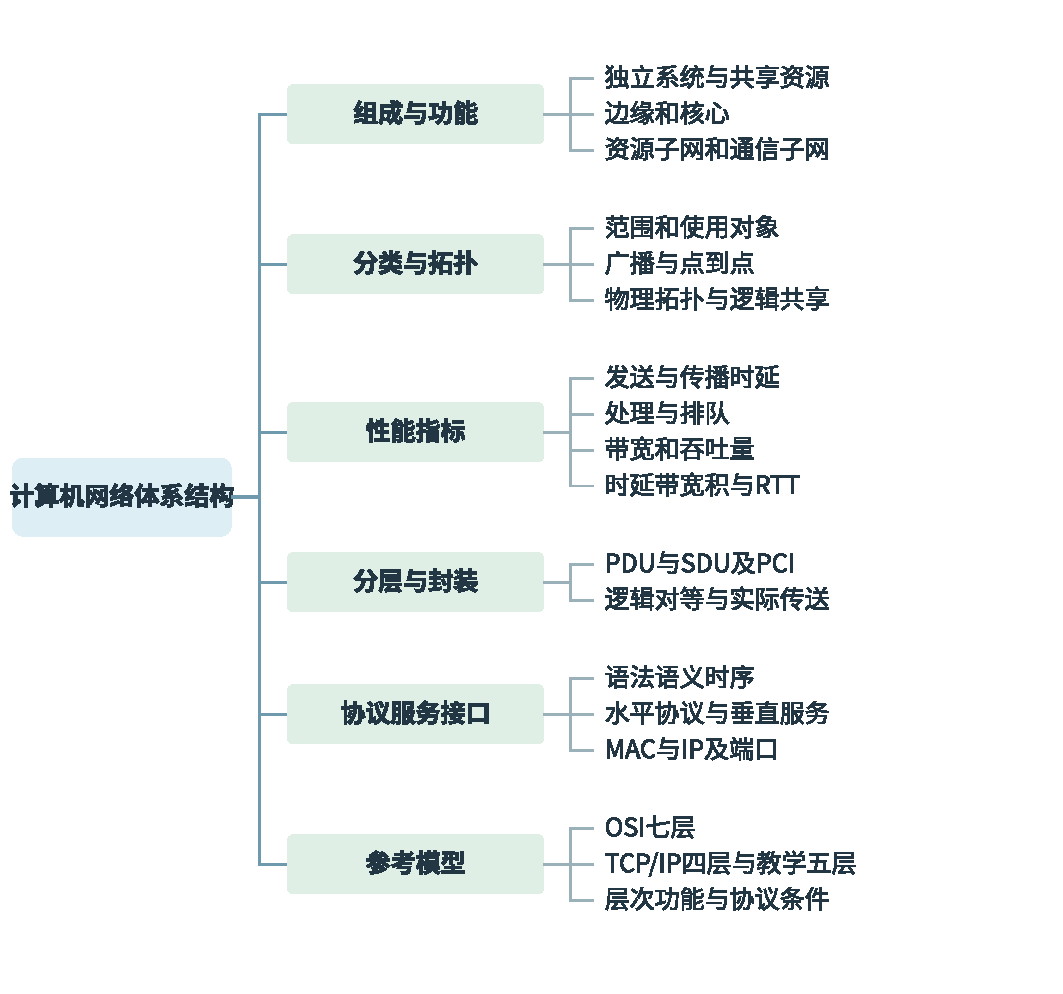
\includegraphics[width=\linewidth,height=168mm,keepaspectratio]{figures/map-01.pdf}\end{wideblock}\par\medskip\clearpage

\par\medskip\noindent\textbf{知识导图（续）}\par\smallskip
\begin{wideblock}\centering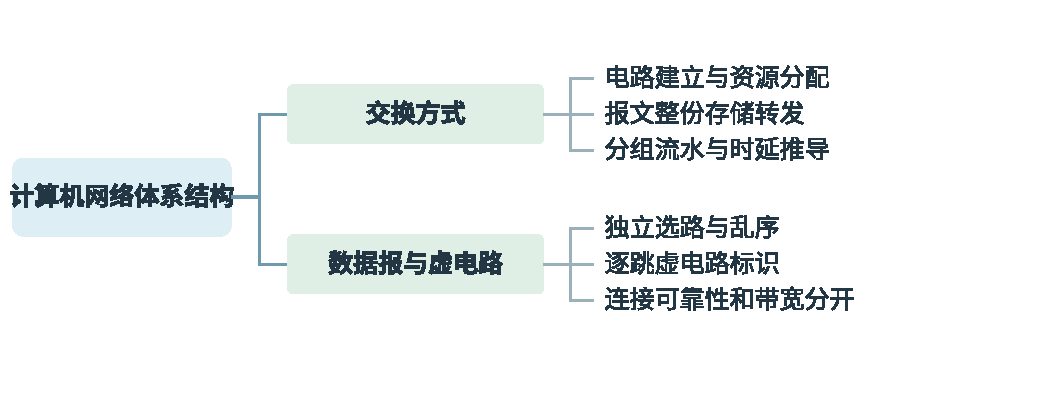
\includegraphics[width=\linewidth,height=168mm,keepaspectratio]{figures/map-02.pdf}\end{wideblock}\par\medskip\clearpage

研究一次网络通信，先固定三个问题：数据从哪个端点到哪个端点，正在观察哪一层，时间从哪一个事件算起。同一个``地址''``确认''或``带宽''，在不同端点、不同层次上所指并不相同；端点与层次确定之后，含义才明确。

本书速率中的 \(\mathrm{k},\mathrm{M},\mathrm{G}\) 分别表示 \(10^3,10^6,10^9\)；1 B=8 bit。容量题若采用二进制数量级，会明确写 KiB、MiB 或题目原约定。除特别说明，传播时延为单向时延，RTT 表示往返时间。

\section{网络由什么组成，提供什么能力}\label{CN01-01}

\begin{definition}[计算机网络]

\textbf{计算机网络}是把具有独立功能的计算设备通过通信链路和网络设备连接起来，按共同协议实现通信与资源共享的系统。这里的独立功能说明设备不是只能依赖某一中央处理机工作的被动终端；共同协议保证发送方表达的格式、动作和次序能够被接收方理解。

\end{definition}

从使用者看，网络提供数据通信、软硬件资源共享、分布式处理等能力。文件放在远端仍可访问，是资源共享；多台机器分工完成计算，是分布式处理。增加通信路径或服务副本可以提高可用性，但``接入网络''本身不保证任何设备都不会失效。

从工作方式看，\textbf{边缘部分}包括用户直接使用的端系统和应用，\textbf{核心部分}由互联的网络与路由设备组成，负责在端系统之间传送分组。从功能分工看，还可区分资源子网与通信子网：前者侧重计算、存储和共享资源，后者侧重数据传送。两种划分的观察角度不同，因此不要把``边缘''机械地等同于某一物理机房。

链路连接相邻节点，路径由一串链路组成。主机 H1 经 R1、R2 到 H2 的路径有三段链路；R1 和 R2 是中间节点。下文的逐跳确认、路由转发和流水传输都以这一区别为基础。

\section{网络分类与拓扑描述的是哪些维度}\label{CN01-02}

按覆盖范围可区分个人区域网、局域网、城域网和广域网。范围是常用的划分依据，但这些名称并没有统一的公里数界限。局域网通常由一个组织管理，并采用以太网或无线局域网等技术；广域网把较远的网络或节点相连，常包含运营商提供的通信服务。

按传输方式可分为广播式与点到点式网络。广播式网络的多个节点共享传输介质，发送后可能被同一介质上的多个节点接收；点到点链路连接两个端点。IP 广播是一种目的地址语义，能转发 IP 广播并不说明设备工作在共享介质上。

\textbf{拓扑}描述节点及链路的连接关系。总线共享一条主干，星形把节点接到中央设备，环形构成闭环，网状提供多条连接。物理星形与逻辑共享介质可以同时成立：集线器外观上是星形连接，内部仍把比特转送到其他端口，各站共享一个冲突域。交换机同样可组成物理星形，但各端口可以并行工作。判断性能时，还要看中央设备工作在哪一层，不能只看画出的形状。

按使用对象还可分公用网与专用网，按介质可分有线网与无线网。这些分类相互独立，一张专用网完全可以同时包含无线局域网和有线广域链路。

\section{发送、传播、排队：怎样确定时延}\label{CN01-03}

长度为 \(L\) bit 的数据经速率为 \(R\) bit/s 的链路发送，\textbf{发送时延}为

\[t_{\mathrm{tx}}=\frac{L}{R}.\]

这段时间从第一位比特进入链路算起，到最后一位比特进入链路为止。提高速率会缩短这段时间，改变距离不会。信号在长度为 \(d\)、传播速度为 \(v\) 的链路上走完所需的\textbf{传播时延}为

\[t_{\mathrm{prop}}=\frac{d}{v}.\]

传播时延描述同一个比特从链路一端移动到另一端所需的时间。数据变短不会使单个比特传播得更快。若没有排队、处理等开销，接收方收到整个数据的时刻是 \(t_{\mathrm{tx}}+t_{\mathrm{prop}}\)，因为最后一位也要走完整段链路。

中间设备检查首部、选择出口需要时间；分组等待处理、等待输出链路空闲，都会产生排队时间。逐跳总时延应按题意累加各段的发送、传播、处理和排队时间。有流水重叠时，不能把``每个分组独立走全程''的时延乘以分组数，本章后续沿时间线计算。

\textbf{带宽}在链路性能题中通常表示额定数据速率；\textbf{吞吐量}表示某一观察区间内实际成功传送的数据率；\textbf{有效吞吐量}只计应用需要的有效载荷。100 Mb/s 链路不等于应用每秒一定能得到100 Mb，首部、确认、竞争和重传都会消耗时间。若一条路径各链路分别为100、10、50 Mb/s，长期单流吞吐量不可能超过10 Mb/s；多个流竞争时还可能更低。

\textbf{时延带宽积} \(R t_{\mathrm{prop}}\) 的单位是 bit，表示在链路持续被填满时，沿一个方向正在传播的比特数量。可靠传输若要让发送方不因等待确认而停顿，更常用 \(R\cdot RTT\) 估算往返期间需要容纳的在途数据量。前者采用单向传播时间，后者采用往返反馈时间，不能在同一公式里不加说明地互换。

\begin{methodbox}[性能题先固定边界]

先写数据量与速率单位，明确问第一位还是最后一位、单向传播还是往返反馈；再在路径上标记存储转发时刻。单链路发送与传播可前后相接，多组多跳可能重叠，不能把一组总时间直接乘组数。

\end{methodbox}

\subsection{一个可直接检查单位的小例}\label{CN01-sub01}

1500 B 分组经100 Mb/s、长200 km 的链路发送，传播速度取 \(2\times10^8\) m/s。发送时延为 \(1500\times8/10^8=120\ \mu s\)，传播时延为 \(200000/(2\times10^8)=1\) ms，最后一位的到达时刻为1.12 ms。链路中的单向时延带宽积为100000 bit，即12.5 kB，已经大于这个分组的长度。链路足够长时，``发送已结束但分组仍在路上''完全可能。

若改用1 Gb/s，传播时延仍是1 ms，发送时延降为12 μs。此例区分三个会独立变化的量：文件有多大、比特送入链路有多快、比特沿介质走多远。

\section{分层与封装：对等层怎样交换数据}\label{CN01-04}

一台主机要把应用数据送出，既要说明应用的含义，又要标识收发进程、选择网络路径、组织一跳传送和产生物理信号。分层把这些任务按相对独立的功能划开。上层调用下层提供的服务，而不需要知道该服务内部采用哪一种队列或硬件实现。

第 \(n\) 层的协议数据单元称为 \(n\) 层 PDU。交给该层的上层数据是其服务数据单元 SDU；该层附加的首部、必要时还有尾部，包含协议控制信息 PCI。常见封装关系为

\[n\text{-PDU}=n\text{-PCI}+n\text{-SDU}.\]

这里``+''表示封装组合：PCI 不一定只出现在首部，也不一定是一段连续字段。上层的 PDU 成为下层的 SDU。接收端按相反方向解封装：先取出本层需要的信息并检查，再把数据向上交付。

\par\medskip\noindent\begin{minipage}{\linewidth}
\centering
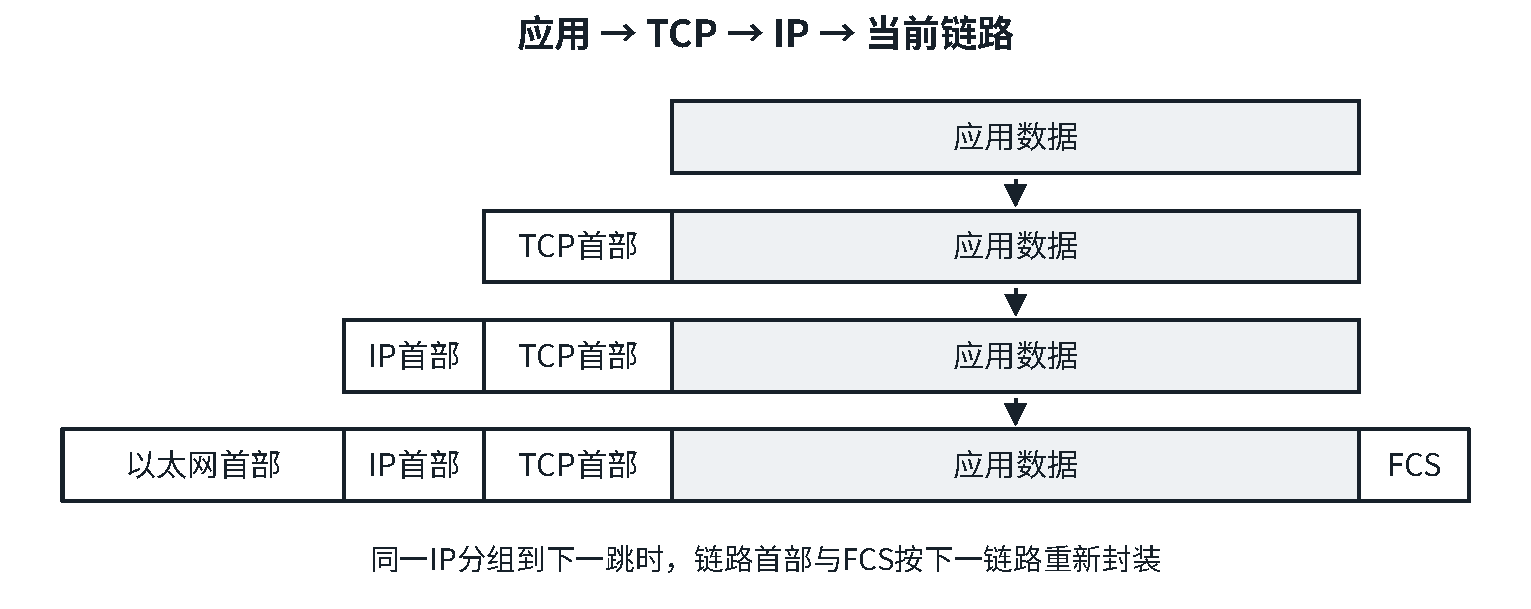
\includegraphics[width=\linewidth,height=125mm,keepaspectratio]{figures/CN01_encapsulation.pdf}
\captionof{figure}{应用数据逐层封装；链路首尾部只用于当前一跳}\label{cn-fig-encapsulation}
\end{minipage}\par\medskip

两个主机的传输层按 TCP 规则进行逻辑上的对等通信，但 TCP 段实际仍须交给本机 IP、链路层和物理层传送。图中的水平联系描述协议关系，竖直联系描述同一节点内的服务调用。普通路由器检查转发所需的网络层信息，不把经过它的每个 TCP 段交给本机应用。

分层能够统一术语、规定接口、减少功能间依赖，\textbf{不要求把各层内部实现算法一并固定}。判断``体系结构是否规定某内容''时，先区分必须遵守的外部行为与具体实现方法。〖1.2-001〗所考的``定义功能执行的方法''属于后者，不能把标准化理解成所有机器必须使用同一种程序。

\section{协议、服务和接口分别约束谁}\label{CN01-05}

\textbf{协议}是对等实体通信时共同遵守的规则，包括语法、语义与时序。语法规定字段格式；语义规定字段与控制信息表示什么、接收后做什么；时序规定什么时候能执行、事件应按何种次序发生。只列出报文的字段，还没有给出完整协议。

\textbf{服务}是本层与下层协作后向上层提供的能力。\textbf{接口}描述同一节点内相邻层如何使用该能力；服务访问点 SAP 是访问服务的位置。协议是水平关系，服务与接口是相邻层的垂直关系。端口是传输层中区分应用端点的标识，MAC 地址、IP 地址和端口各属不同层次，不能把三者互相替代。

把同一次普通通信放在三个层次比较，先问``这个标识交给谁解释、它指向哪一种端点''，再看它会不会随转发改变。

\begin{wideblock}

\par\medskip\noindent\begin{minipage}{\linewidth}\fontsize{9.3}{12}\selectfont\begin{tabularx}{\linewidth}{@{}YYYY@{}}
\toprule\noalign{}
\begin{minipage}[b]{\linewidth}\raggedright
比较项
\end{minipage} & \begin{minipage}[b]{\linewidth}\raggedright
以太网MAC地址
\end{minipage} & \begin{minipage}[b]{\linewidth}\raggedright
IPv4地址
\end{minipage} & \begin{minipage}[b]{\linewidth}\raggedright
TCP/UDP端口
\end{minipage} \\
\midrule\noalign{}


所在首部与长度 & MAC帧头，源、目的各48 bit & IPv4首部，源、目的各32 bit & 传输层首部，源、目的各16 bit \\
基本指向 & 当前以太网一跳的收发接口 & IP分组的源与目的主机接口 & 对应主机上的应用端点 \\
谁据此作基本处理 & 网卡接收、二层交换机查目的MAC转发 & 路由器按目的IP查路由 & 目的主机传输层分用 \\
普通跨路由转发 & 下一跳重新封装源、目的MAC & 不经NAT时源、目的通常保持 & 不经端口转换时源、目的通常保持 \\
\bottomrule\end{tabularx}
\end{minipage}\par\medskip

\end{wideblock}

表中关于MAC地址的结论只适用于普通以太网；802.11还要区分当前无线跳与原始源/目的。路由器收到的帧，目的MAC可以是自己，其中IP分组的目的地址却仍是远端主机。因此``这一层收到数据''不等于``最终应用已收到数据''。第3～5章的格式图会把这些标识放回各自首部。

还要把``建立连接''``可靠交付''``有确认''分开判断。面向连接服务在传送前建立逻辑联系，通常需要保留状态；无连接服务让各数据单元独立提交。可靠服务承诺按其定义处理丢失、重复、次序等问题；有确认只说明存在应答机制。连接不等于预留固定带宽，检错不等于可靠交付，一次确认也不能独自解决重复接收。

这三个问题应分别作答：虚电路先建立逻辑路径，是否可靠还要看具体协议；以太网有CRC检错，基本MAC却没有逐帧确认重传；802.11的单播确认只反馈当前无线跳，不能证明远端应用交付。比较服务时固定端点和协议，才能避免把一项机制扩成整条通信路径的保证。

\section{OSI 与 TCP/IP：先看模型，再看端点}\label{CN01-06}

OSI 自下而上为物理层、数据链路层、网络层、传输层、会话层、表示层、应用层。它把功能关系抽象出来，不是要求现实网络的每个设备都有七层独立软件。

\begin{wideblock}

\par\medskip\noindent\begin{minipage}{\linewidth}\fontsize{9.3}{12}\selectfont\begin{tabularx}{\linewidth}{@{}YYY@{}}
\toprule\noalign{}
\begin{minipage}[b]{\linewidth}\raggedright
层次
\end{minipage} & \begin{minipage}[b]{\linewidth}\raggedright
判断功能时先找的对象
\end{minipage} & \begin{minipage}[b]{\linewidth}\raggedright
典型任务
\end{minipage} \\
\midrule\noalign{}


物理层 & 一段物理链路上的原始比特 & 电平、编码、接口、比特传输 \\
数据链路层 & 相邻节点之间的帧 & 成帧、检错、按协议实现流控与可靠传输、介质访问 \\
网络层 & 跨网络传送的分组 & 寻址、路由选择与转发 \\
传输层 & 不同主机上的应用进程端点 & 复用分用、按协议实现可靠传输与流控 \\
会话层 & 应用之间的会话 & 对话管理、同步点与恢复 \\
表示层 & 数据的表示方式 & 编码格式转换、压缩与加密 \\
应用层 & 应用所需的网络功能 & Web、邮件、名称服务等 \\
\bottomrule\end{tabularx}
\end{minipage}\par\medskip

\end{wideblock}

数据链路层与传输层都可能包含流量控制，区分依据是控制范围。相邻节点之间，接收方来不及处理帧，是链路层问题；两个端系统之间，接收进程处理不及，是传输层问题。噪声使比特翻转属于物理传输现象，是否发现差错、是否重传，则要看上层协议，不能由``差错发生在物理链路''推出``物理层完成全部差错控制''。

\subsection{例 1-1　端到端服务从哪层开始}\label{CN01-ex1}

\begin{example}[配套例题]

配套例题。 在 OSI 参考模型中，自下而上第一个提供端到端服务的层次是（　）。

A. 数据链路层　B. 传输层　C. 会话层　D. 应用层

\end{example}

\textbf{解析。} ``自下而上第一个''要求找到跨越中间网络、服务于两端应用进程的最低层次。数据链路层只处理相邻节点，网络层把分组送到目的主机；传输层开始为进程端点提供服务。因此选 \textbf{B}。会话层、应用层也工作在端系统，但都不是题目所问的第一个层次。

\subsection{例 1-2　相邻节点间的流量控制}\label{CN01-ex2}

\begin{example}[配套例题]

配套例题。 在 ISO/OSI 参考模型中，实现两个相邻结点间流量控制功能的是（　）。

A. 物理层　B. 数据链路层　C. 网络层　D. 传输层

\end{example}

\textbf{解析。} 题干已经把范围限定为``相邻结点间''，应在帧的一跳交付层次判断，选 \textbf{B}。若条件改成两端主机中应用进程间的流量控制，应转到传输层；不能只背``流控属于某一层''。

TCP/IP 常用四层模型为网络接口层、网际层、传输层、应用层。网络接口层对应具体链路技术，网际层以 IP 实现尽最大努力的数据报交付，传输层包括 TCP 与 UDP，应用层合并 OSI 上三层的任务。本书为展开链路机制，把网络接口层再分为数据链路层、物理层，采用五层教学表示；五层与四层模型的分界不同，但协议关系不变。

还应区分抽象模型中允许的功能与某种实际协议提供的服务。OSI 网络层可以讨论面向连接和无连接服务；现实 IP 提供无连接服务。以太网帧含 FCS，但通常检测到错误后丢弃，不负责链路层确认重传；不能把``链路层可提供可靠传输''写成``所有链路层协议保证无差错、有序交付''。TCP/IP 的传输层同时有 TCP、UDP，也不能拿 UDP 直接回答只针对教材 OSI 模型约定的题。

\section{电路、报文和分组交换如何沿时间线计算}\label{CN01-07}

\textbf{电路交换}先建立端到端电路，通信期间按分配的资源传送，结束后释放。其完成时间通常包括建立时间、源端发送时间和沿路径传播时间；电路一旦建立，中间节点就不必收全整份文件再重新发送。电路在空闲时仍可能保留资源。

\textbf{报文交换}把一整份报文作为存储转发单位；中间节点收全报文后才能向下一段链路发送。\textbf{分组交换}把报文切成较小分组，每组独立存储转发，因此不同链路可以同时传送不同分组。分组需要附加首部，且可能排队、丢失或乱序；``分成越小越快''忽略了首部和处理代价。

比较三种方式，要放在同一条时间线上：什么时候可以开始，中间节点要等多少数据，链路空闲时资源能否供别人使用。

\begin{wideblock}

\par\medskip\noindent\begin{minipage}{\linewidth}\fontsize{9.3}{12}\selectfont\begin{tabularx}{\linewidth}{@{}YYYY@{}}
\toprule\noalign{}
\begin{minipage}[b]{\linewidth}\raggedright
比较维度
\end{minipage} & \begin{minipage}[b]{\linewidth}\raggedright
电路交换
\end{minipage} & \begin{minipage}[b]{\linewidth}\raggedright
报文交换
\end{minipage} & \begin{minipage}[b]{\linewidth}\raggedright
分组交换
\end{minipage} \\
\midrule\noalign{}


传送前准备 & 先建立电路并分配资源 & 可直接提交报文 & 数据报可直接提交；虚电路另需建立逻辑路径 \\
中间节点的基本转送单位 & 已建立电路中的比特流 & 完整报文 & 一个分组 \\
开始向下一段发送的条件 & 电路已接通，可连续传送 & 收齐整个报文且出口可用 & 存储转发模型下收齐该分组且出口可用 \\
资源使用 & 分配给连接的资源在空闲时也可能保留 & 链路按报文动态共享 & 链路按分组动态共享，可形成流水 \\
时间与存储的主要代价 & 建立时间、专用资源占用 & 长报文逐跳收齐的等待与缓存 & 分组首部、排队与处理；小组过多会增加开销 \\
\bottomrule\end{tabularx}
\end{minipage}\par\medskip

\end{wideblock}

由此可见，完成时间的先后没有固定顺序，必须结合具体条件判断。短数据可能来不及抵消建立电路的开销；长数据可从分组流水获益，但首部与排队又会影响结果。题目给出直通等转发规则时，还需修改``收齐才转发''的事件条件，不能同时套用存储转发公式。

\par\medskip\noindent\begin{minipage}{\linewidth}
\centering
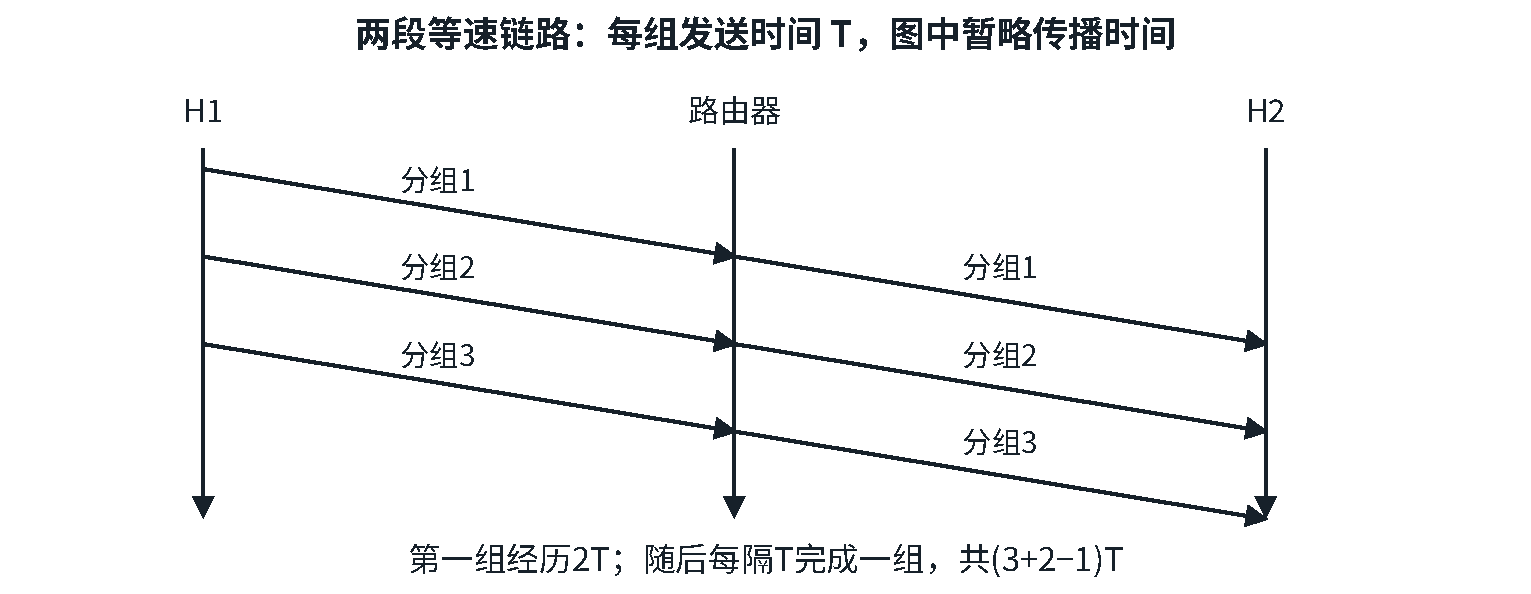
\includegraphics[width=\linewidth,height=125mm,keepaspectratio]{figures/CN02_packet_pipeline.pdf}
\captionof{figure}{两段等速链路上的三个分组；箭头连接本组开始发送与下一节点收齐的时刻，并非单个比特的传播线}\label{cn-fig-pipeline}
\end{minipage}\par\medskip

若有 \(h\) 段等速链路、每组总长 \(L\) bit、速率 \(R\)，共 \(n\) 个等长分组，无排队和处理开销，第一组需 \(hL/R\) 完成发送，后续每组间隔 \(L/R\) 到达，故

\begin{theorem}[等速存储转发流水的完成时间]

在上述等长分组、固定等速路径、无竞争及处理开销的模型下，

\[T=(n+h-1)\frac{L}{R}+\sum_{i=1}^h t_{\mathrm{prop},i}.\]

\end{theorem}

第一组要在每段链路完整发送一次，所以发送项为\(hL/R\)；流水填满后，每个出口每隔\(L/R\)送完下一组，后续\(n-1\)组只再增加\((n-1)L/R\)。沿途固定传播项对首组累加，后续相邻组间隔不再重复加入整条路径传播时间，得到上式。

若一个报文长 \(F\) bit，按整报文存储转发，则相应发送项为 \(hF/R\)。链路速率不同时，先按各链路的开始与结束事件递推，不能随意把 \(R\) 换成平均速率。对等长分组、固定路径和无其他流量的理想流水，第一组时延之后，后续组受最慢链路的服务间隔限制。

\subsection{例 1-3　时延带宽积先转成传播时间}\label{CN01-ex3}

\begin{example}[配套例题]

配套例题。 在下图所示的分组交换网络中，主机 H1 和 H2 通过路由器互连，2段链路的带宽均为100 Mb/s，时延带宽积（即单向传播时延\ensuremath{\times}带宽）均为1000 bit。若 H1 向 H2 发送1个大小为1 MB的文件，分组长度为1000 B，则从 H1 开始发送时刻起到 H2 收到文件全部数据时刻止，所需的时间至少是（注：\(M=10^6\)）（　）。

\par\medskip\noindent\begin{minipage}{\linewidth}
\centering
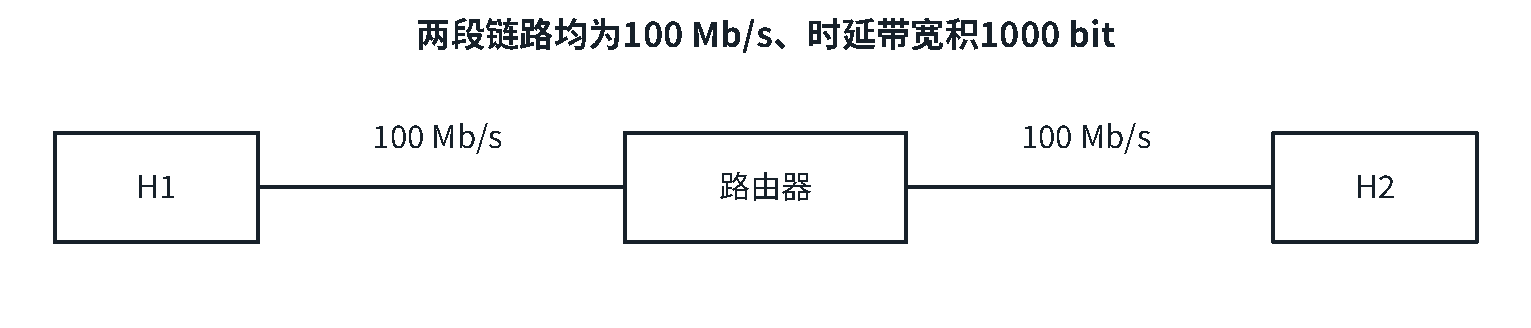
\includegraphics[width=\linewidth,height=125mm,keepaspectratio]{figures/CN15_two_links_2023.pdf}
\captionof{figure}{原题的两段链路，均为100 Mb/s且时延带宽积1000 bit}\label{cn-fig-2023links}
\end{minipage}\par\medskip

A. 80.02 ms　B. 80.08 ms　C. 80.09 ms　D. 80.10 ms

\end{example}

\textbf{解析。} 按题设分组长度直接切分文件，分组数为 \(10^6/1000=1000\)，每组发送时间为 \(8000/10^8=80\ \mu s\)。每段传播时间由时延带宽积求得 \(1000/10^8=10\ \mu s\)。

两段链路上第一组用 \(2\times80+2\times10=180\ \mu s\) 到齐；后续999组每隔80 μs到齐。总计

\[180+999\times80=80100\ \mu s=80.10\text{ ms},\]

选 \textbf{D}。1000个分组并不是各自独占两段链路、依次走完全程，因此不能算成 \(1000\times180\ \mu s\)。本题没有额外给出分组首部，不要自行把每组1000 B再增加20 B。

\section{数据报与虚电路：连接不等于电路}\label{CN01-08}

数据报方式让每个分组独立携带寻址信息、独立选择下一跳。同一报文的分组可能走不同路径，可能乱序；IP属于这种方式。网络不保证交付，并不妨碍端系统在其上建立 TCP 可靠连接。

虚电路方式先建立一条逻辑路径，在各中间节点保存映射状态。分组到达某节点后，按输入链路及虚电路标识查出输出链路和新的局部标识。VCID通常具有链路局部意义，不要求一路数值不变。按既定路径转发有利于保持分组顺序，但是否提供检错重传、带宽保障，仍取决于具体服务。

按相同的维度比较两者：数据报在每组中带目的寻址信息，网络不为这次通信预建逐跳虚电路状态，每组可独立选路；虚电路在建立时选路并保存映射，后续组按局部VCID转发。同一路径、较短标识和按序到达是虚电路模型的特点，资源是否独占却不是由``有连接''决定的。电路交换与虚电路都可能先建立联系，前者分配电路资源，后者仍把链路按分组共享。

\subsection{例 1-4　虚电路必须预留带宽吗}\label{CN01-ex4}

\begin{example}[配套例题]

配套例题。 下列关于虚电路网络的叙述中，错误的是（　）。

A. 可以确保数据分组传输顺序

B. 需要为每条虚电路预分配带宽

C. 建立虚电路时需要进行路由选择

D. 依据虚电路号（VCID）进行数据分组转发

\end{example}

\textbf{解析。} 虚电路建立了路径与转发状态，但依然属于分组交换；多条虚电路可以共享链路，不必各自占用一份固定带宽。错误项为 \textbf{B}。建立时选路、传送时按已建状态转发，与``每个分组重新独立选路''的数据报方式不同。永久虚电路可以长期保留，不能说所有虚电路都在一次会话后立即撤销。

\section{主动回忆自测}\label{CN01-review}

以下为自拟回顾题。先遮住答案，按导图主枝口述条件，再进行数值计算。

\begin{enumerate}
\def\labelenumi{\arabic{enumi}.}
\tightlist
\item
  按工作方式划分的核心/边缘，与按功能划分的通信/资源子网是否完全同义？
\item
  1 MB文件经10 Mb/s、单向传播20 ms的一条链路传送，不计首部和其他开销，最后一位何时到达？
\item
  某帧从交换机端口1进入、端口3出去，能证明远端应用进程已收到数据吗？
\item
  为什么协议描述的是水平关系，服务和接口描述的是垂直关系？
\item
  OSI和TCP/IP的层数不同，能否据此断定其中一个模型没有应用层？
\item
  报文切为10个等长分组，经3段等速链路存储转发；每组发送1 ms、每段传播2 ms，无其他开销，最后一组何时到达？
\item
  虚电路先建立逻辑路径，能否直接推出必须为其预留一份固定带宽？
\item
  收到帧后CRC通过，是否已经证明端到端数据无差错且不会丢失？
\end{enumerate}

\subsection{核对答案}\label{CN01-review-answers}

\begin{enumerate}
\def\labelenumi{\arabic{enumi}.}
\tightlist
\item
  不完全同义，两者分别强调位置/工作方式与承担功能。
\item
  发送0.8 s，传播0.02 s，共0.82 s；不是只算发送时间。
\item
  不能，只能说明当前交换机完成了一次链路层转发，还需后续路径与目的端解封装。
\item
  对等实体共同遵守协议；同机上层调用下层服务，接口约束调用方式。
\item
  不能，TCP/IP应用层合并了OSI上三层的相关任务。
\item
  \((10+3-1)\times1+3\times2=18\) ms；第一组9 ms到齐，之后每组间隔1 ms。
\item
  不能，虚电路仍可以按分组共享链路，资源保证取决于具体协议与服务。
\item
  不能，检验存在漏检，链路检验也不能承诺后续路径可靠交付。
\end{enumerate}

\end{document}
